% !Mode:: "TeX:UTF-8"
%!TEX program  = xelatex

\documentclass{cumcmthesis}
%\documentclass[withoutpreface,bwprint]{cumcmthesis} %去掉封面与编号页
\usepackage{subfig}
\usepackage{url}
\usepackage{amsmath}
\usepackage{wrapfig}
\usepackage{graphics}
\usepackage{graphicx}%图片
\title{meng son}
\tihao{C}
\baominghao{202427004386}
\schoolname{西安电子科技大学}
\membera{孟文堂 \quad 23009101365}
\memberb{谢小凡 \quad 23009100237 }
\memberc{魏朝旭 \quad 23009201082}
\supervisor{冯海林}
\yearinput{2024}
\monthinput{9}
\dayinput{8}

\begin{document}

 \maketitle
 \begin{abstract}
 	
本文针对\textbf{生鲜商超}中蔬菜类商品的自动定价与补货决策问题，运用数据分析、时间序列分析、聚类分析以及优化算法等方法，建立了\textbf{蔬菜销售预测}模型、\textbf{成本加成定价}模型以及利润最大化模型。通过销售数据的统计分析，得到了单品和品类的销售分布规律及其相互关系；通过时间序列分析，识别了销售量的季节性周期；利用K-means++聚类算法，对单品进行了市场细分；最终，通过优化算法（如LINGO和遗传算法）求解出了未来一周的补货总量和定价策略，以及特定日期的单品补货量和定价，较好地解决了商超的\textbf{补货和定价优化}问题。

针对问题一，首先通过计算三年内各单品的总销售量，得到了单品销售分布规律，并取前二十位进行分析；其次，利用系统聚类谱系图和K-means++算法，对单品进行了聚类分析，识别出不同的销售群体；同时，绘制了品类销售量的折线图，揭示了其季节性周期规律；最后，通过\textbf{Spearman相关系数}，计算了各品类之间的相关性，揭示了它们之间的市场关联。

针对问题二，首先计算了每个品类每天的总销售量和加权平均价格，通过曲线拟合建立了销售量和价格的关系函数；然后，利用历史数据预测了未来一周的销售量，并通过关系函数预测了相应的平均价格；最后，构建了\textbf{利润最大化}模型，使用优化算法求解出了各品类的最优补货量和定价策略，实现了商超收益的最大化。

针对问题三，首先预测了7月1日各单品的销售量，然后结合最小陈列量要求和商超销售空间限制，构建了单品补货和定价的优化模型；通过\textbf{遗传算法}求解该模型，得到了满足市场需求且使商超收益最大的单品补货量和定价策略。

针对问题四，为了更好地制定蔬菜商品的补货和定价决策，商超还需要采集实时库存数据、供应商信息、顾客购买行为数据、竞争对手信息以及市场趋势数据等。这些数据有助于商超更准确地预测市场需求、优化库存管理、降低采购成本、提高顾客满意度以及增强市场竞争力。本文所运用的模型优点在于能够综合考虑多种因素，为商超提供科学的决策支持；但同时，模型的准确性和有效性也依赖于数据的完整性和准确性，以及算法的选择和参数设置。因此，在实际应用中，需要根据具体情况对模型进行调整和优化。

\keywords{蔬菜销售预测\quad Spearman相关系数\quad 利润最大化\quad 补货和定价优化\quad 遗传算法}
\end{abstract}

%目录
%\tableofcontents
%\newpage
\section{问题重述}

\subsection{问题背景}

在当今农业持续进步的时代背景下，如何高效且可持续地管理有限的耕地资源，通过优化种植布局来提升农业经济效能，已成为乡村经济可持续增长所必须深入探讨的关键问题。特别是在诸如华北山区等特定地域，鉴于其独特的气候环境、多样化的土地资源构成以及作物生长的特定规律，精心策划农作物的种植策略变得尤为关键。这种规划不仅是对自然条件的适应，更是推动农业可持续发展、增强农村经济活力的必要途径。

\subsection{问题内容}

本研究以华北山区某乡村的农作物种植策略为研究对象，基于历史销售数据、市场趋势预测、农作物生长特性、种植成本及市场价格变动等信息，建立数学模型，以解决以下关键问题：

（1）\textbf{问题一：}在农作物预期销售量、种植成本、亩产量和销售价格均保持稳定的前提下，每季农作物需当季销售完毕。相关数据位于附件1与附件2中，针对两种情况制定2024-2030年农作物种植方案：
\begin{itemize}
\item 情况一：超出预期销售量的部分将滞销，造成浪费。
\item 情况二：超出部分按2023年销售价格的50\%降价处理。
\end{itemize}

分别计算并输出两种情况下的最优种植方案至result1\_1.xlsx和result1\_2.xlsx。

（2）\textbf{问题二：}考虑农作物未来预期销售量、亩产量、种植成本和销售价格的不确定性，其中小麦和玉米预期销售量有增长趋势（5\%-10\%），其他作物预期销售量有±5\%变化；亩产量受气候影响有±10\%变化；种植成本每年增长约5\%；粮食类作物价格稳定，蔬菜类作物价格每年增长约5\%，食用菌价格稳中有降（特别是羊肚菌每年降5\%）。综合考虑上述不确定性及风险，制定2024-2030年农作物的最优种植方案，并输出至result2.xlsx。

（3）\textbf{问题三：}在问题2的基础上，进一步考虑农作物之间的可替代性和互补性，以及预期销售量、销售价格与种植成本之间的相关性。通过模拟数据，综合考虑这些复杂因素，制定2024-2030年农作物的最优种植策略，并与问题2的结果进行比较分析。
\section{问题分析}

\subsection{问题一的分析}

问题一要求我们分析附件1和附件2提供的数据，针对两种情况分别得出从2024年到2030年7年，该村农作物的最优种植方案，即得到使得利润最大的种植方案。针对两种情况我们可以得到两个利润的目标函数，加上题干中每种作物在同一地块（含大棚）都不能连续重茬种植，每个地块（含大棚）的所有土地三年内至少种植一次豆类作物等约束条件。我们可以建立相关优化模型，并代入附件中的相关数据，从而得出最优种植方案。

同时，由于附件中缺少2023年各作物每季的预期销售量，我们需要提前查询相关数据文献，以便模型求解。

\subsection{问题二的分析}

第二问在第一问的基础上增加了对于不确定因素与风险因素等的考虑，预期销售量、农作物亩产量、销售价格和种植成本等指标转变为波动变量，在一定区间内变化。问题从本质上属于不确定性条件下的优化问题。大部分条件数据变化范围明显，题目中已经告知。而潜在种植风险则要综合考虑一些其他因素，譬如：自然风险，运输风险等等。这些潜在风险则需要查询相关数据，进一步对目标函数进行约束。

\subsection{问题三的分析}

问题三已经指出预期销售量、销售价格与种植成本之间存在一定相关性。那么意味着可以对数拟合或者其他方法去尝试拟合出三者中两两之间的函数关系。有了数值关系后，再在问题二的基础上综合考虑。我么假定种植成本选取问题二所使用的个农作物成本。那么由于函数关系的存在，问题二中动态浮动的预期销售量和销售价格也会变得相对稳定，即两者的数值此时是由种植成本所决定的，即题干中的模拟数据。此时再去用问题而的模型决策出最优策略，由于相应农作物相关数据与第二问发生了改变，最优策略也将发生改变。

因为拟合函数本质是考虑进去了各种农作物的可替代性和互补性，预计此时最优种植策略相比于第二问的种植策略，逐年相比总利润是增加的。具体情况，需要在模型求解后具体分析。


\section{模型的假设}

\begin{itemize}
\item 	假设34个地块每季只单种一种作物，以满足每种作物在单个地块种植面积不宜太小，同时方便管理的需求，并简化模型。
\item 	假设每个大棚可以等分成两个单位，每个单位每季只能种植一种植物，20个大棚则可以分成40个单位。借此既满足每种作物在单个地块种植面积不宜太小并方便管理的需求，又能保证大棚的利用效率。对于分成两个单位的大棚编号，分别加上第二个角标1或2进行区分，比如大棚E1划分为E11和E12区域。
\item  假设题干所述华北地区该地一切贸易仅考虑国内市场，因为该地处于华北山区农村地带，销量小，无法有有效的渠道进入国际贸易市场。
\item 	忽略2023年以前各作物,尤其是豆类的种植情况，以简化模型。
\item   假设华北地区潜在种植风险只考虑自然风险，并且可以量化。
\end{itemize}
\section{符号说明}

对文中所用到的符号加以阐述和说明，如表~\ref{tab001}~所示。
\begin{table}[!htbp]
	\caption{符号说明}\label{tab001} \centering
	\begin{tabular}{cccccccccc}
		\toprule[1.5pt]
		符号 &  &  &  &  & & & &  & 说明\\
		\midrule[1pt]
		$t$ &  &  &  &  &  & & & & 年份\\
		$s$ &  &  &  &  &  &  & & & 各种类型地的面积\\
		$k$ &  &  &  &  &  &  & & & 地的种类编号\\
		$x$ &  &  &  &  &  &  & & & 作物的种类编号\\
		$W$ &  &  &  &  &  &  & & & 利润\\
		$\text{Sale}$ &  &  &  &  &  &  & & & 预期销售量矩阵\\
		$\text{Price}$ &  &  &  &  &  &  & & & 销售价格矩阵\\
		$\text{Yield}$ &  &  &  &  &  &  & & & 亩产量矩阵\\
		$\text{Field}$ &  &  &  &  &  &  & & & 土地规划矩阵\\
		$\text{Cost}$ &  &  &  &  &  &  & & & 种植成本矩阵\\
		

		\bottomrule[1.5pt]
	\end{tabular}
\end{table}

\section{模型的建立与求解}

\subsection{问题一的模型建立与求解}

\subsubsection{数据处理}
\textbf{1.获取作物预期销售量数据}

由于附件中缺少2023年各作物每季的预期销售量，我们首先进行农产品预期销售量的测算。预期销售量，即人们对作物的需求量。因为地处华北山区村庄，销量较小，没有较好的渠道进入国际贸易，所以我们只考虑国内市场的需求。

粮食自给率是一项评估国家粮食自给程度的指标，用总产量/（总产量+进口量-出口量）定义。通过判断自给率是否大于1，可以分为两种情况：

\begin{itemize}
	\item 	当自给率>100\%时,净出口量即为国内市场的农作物滞销量，滞销率=滞销量/总产量。
	\item 	当自给率<100\%时,总产量=预期销售量，滞销率为0。
\end{itemize}

总产量抛去滞销量，那么剩下的就是预期销售量，即预期销售量=产量$\times$(1-滞销率)。

从《中国统计年鉴(2023)》	得到薯类、高粱等粮食类以及菜和食用菌相关数据\cite{bib:one}，置于\underline{附录B}中。最终得到粮食类农作物自给率为86.26\%,滞销率为0，菜及食用菌类农作物自给率为101.09\%，滞销率为1.08\%。从而得到作物的预期销售量。

\textbf{2.初始化各种数据矩阵及规划矩阵表示形式}

通过附件中信息的获取，我们最终的得到了	$\text{Sale},\text{Price},\text{Yield},\text{Cost}$四种矩阵的初始数据。四种矩阵形式上都是$41 \times 6$，分别对应41种作物在六类地形(包括大棚)中对应的统计量，矩阵每一行都代表一个作物。相关统计数据置于\underline{附录C}中。

对于最终模型结果的规划矩阵，我们用$\text{Field}$矩阵表示，如下：

$$
\text{Field}=
\begin{bmatrix}
	x_{1,1}  &0   &0  &0  &s  &k \\
	x_{2,1}  &0   &0  &0  &s  &k \\
	\vdots  &\vdots  &\vdots  &\vdots  &\vdots  &\vdots \\
	x_{m,1}&  x_{m,2}& x_{m,3} &x_{m,4}  & s & k\\
	\vdots &  \vdots & \vdots  &  \vdots &  \vdots & \vdots \\
	x_{54,1}&  x_{54,2}& x_{54,3} & x_{54,4} &s  &k
\end{bmatrix}
$$


其中，x为作物的种类编号，s为地的面积，k为地的种类编号。
\subsubsection{模型建立}
\textbf{1.约束条件}


	(1) 平旱地、梯田和山坡地每年都只能种植一季作物。
	
	(2) 水浇地每年可以种植一季也可以种植两季作物。
	
	(3) 大棚能够在一定程度上起保温作用，每年都可以种植两季作物。
	
	(4) 智慧大棚主要是在冬季利用太阳能自动调节棚内温度，保证作物的正常生长。

	(5) 平旱地、梯田和山坡地每年适宜单季种植粮食类作物（水稻除外）。
	
	(6) 水浇地每年可以单季种植水稻或两季种植蔬菜作物。
	
	(7) 若在某块水浇地种植两季蔬菜，第一季可种植多种蔬菜（大白菜、白萝卜和红萝卜除外）；第二季只能种植大白菜、白萝卜和红萝卜中的一种（便于管理）。
	
	(8) 根据季节性要求，大白菜、白萝卜和红萝卜只能在水浇地的第二季种植。
	
	(9) 普通大棚每年种植两季作物，第一季可种植多种蔬菜（大白菜、白萝卜和红萝卜除外），第二季只能种植食用菌。
	
	(10) 因食用菌类适应在较低且适宜的温度和湿度环境中生长，所以只能在秋冬季的普通大棚里种植。
	
	(11) 智慧大棚每年都可种植两季蔬菜（大白菜、白萝卜和红萝卜除外）。

	(12) 每种作物在同一地块(含大棚)都不能连续重茬种植，即$\text{Field}(t)!=\text{Field}(t-1)$。
	
	(13)因含有豆类作物根菌的土壤有利于其他作物生长，从2023年开始要求每个地块(含大棚)的所有土地三年内至少种植一次豆类作物，即$\text{Field}(t),\text{Field}(t-1),\text{Field}(t-2)$中存在对应可种植的豆类食物。
	
	
	对于以上(1)-(4)条隐含的约束条件在规划矩阵$\text{Field}$的结构设置中已经囊括，无需额外进行显式限制条件的增加。同时，题干中对于每种地形存在据具体的种植限制，主要有(5)-(11)7条约束，我们将在具体计算中加以限制。此外，根据作物的生长规律，对于相邻年份来说作物种植会有所影响。所以产生了(12)(13)两条约束。
	
	\textbf{2.目标函数}
	
	由于题干要求分析两种特定情况下的最优方案，即保证它们的利润最大。故分别列出两种情况的目标函数：
	
	$$
	W_1=\sum_{i}^{54} \sum_{j}^{4}min(\frac{ \text{Yield}_{m,n} \times \text{Field}_{i,5}}{2} ,\text{Sale}_{m,n}
	)\times \text{Price}_{m,n}-\frac{ \text{Cost}_{m,n}\times \text{Field}_{i,5}}{2}   
	 $$
	
\begin{equation*}
	\begin{split}
		W_2&=\sum_{i}^{54} \sum_{j}^{4}min(\frac{ \text{Yield}_{m,n} \times \text{Field}_{i,5}}{2} ,\text{Sale}_{m,n}
		)\times \text{Price}_{m,n}-\frac{ \text{Cost}_{m,n}\times \text{Field}_{i,5}}{2} \\ &+\left|\frac{ \text{Yield}_{m,n} \times \text{Field}_{i,5}}{2} -\text{Sale}_{m,n} \right |
		\times \frac{\text{Price}_{m,n}}{2}
	\end{split}
\end{equation*}


	其中，$m=\text{Field}_{i,j},n=\text{Field}_{i,6}$。
	
	\textbf{3.模型建立}
	
\begin{wrapfigure}{l}{8.5cm}
	
	\centering
	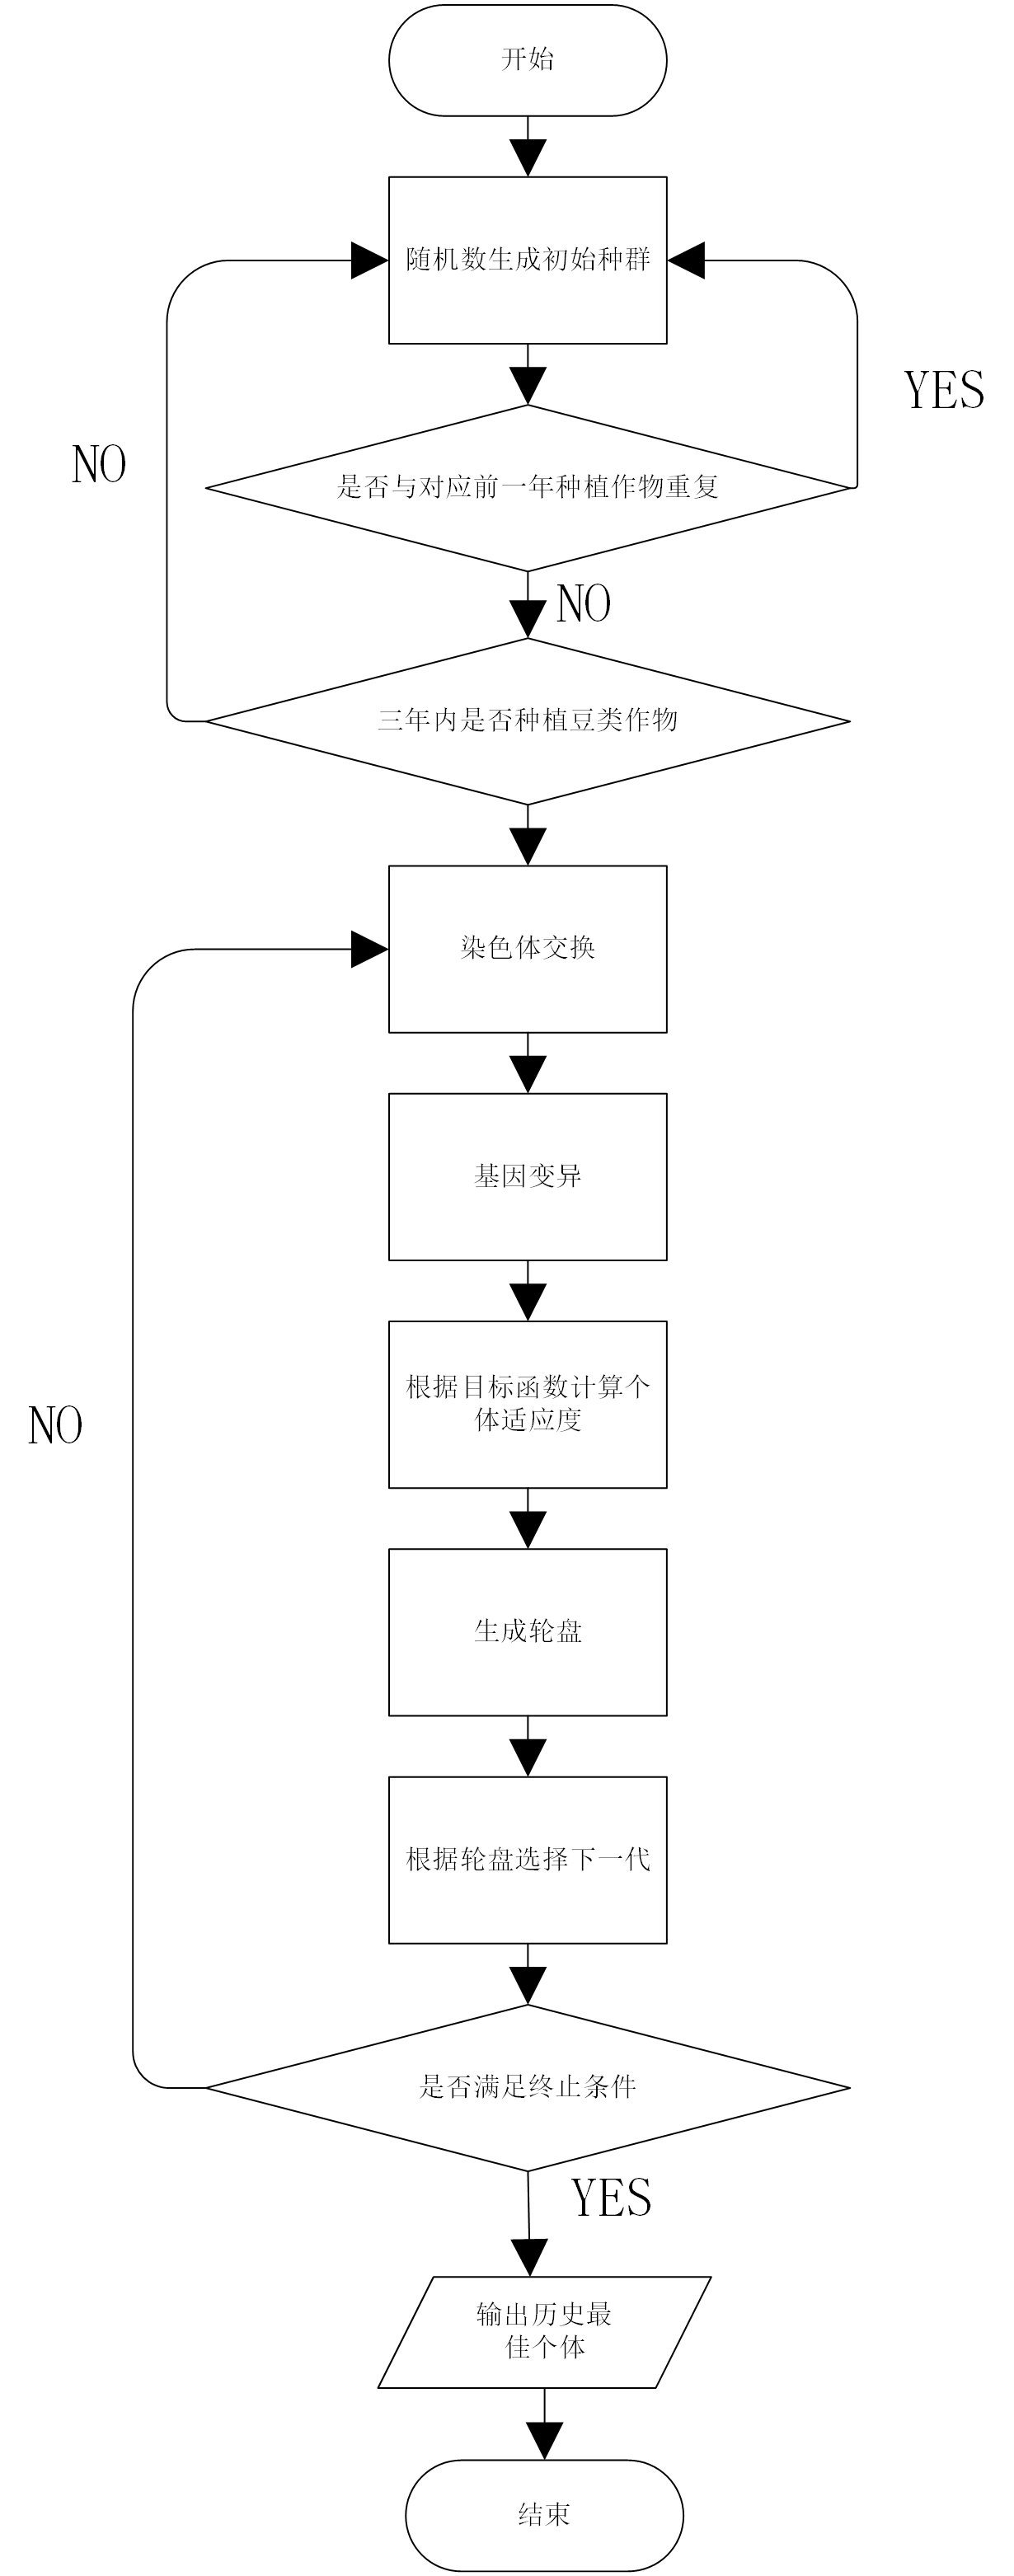
\includegraphics[width=7cm]{figures/遗传算法.png}
	\caption{遗传算法模型流程图 }\label{img001}
\end{wrapfigure}

我们将该问题视为一道优化问题，选择采用遗传算法进行求解，通过模拟生物进化过程进行交叉变异等操作以得到最优解。,具体思路如图~\ref{img001}~所示。

创建初始种群个体时，通过设置限制：

(1)$\text{Field}(t)!=\text{Field}(t-1)$;

(2)$\text{Field}(t),\text{Field}(t-1),\text{Field}(t-2)$中存在对应可种植的豆类食物。

以实现同一种作物不可连续在同一地块连续种植的约束且同一地块三年内必至少种植一次豆类作物。

此外，通过对不同地块情况的分类讨论，添加相应的限制条件，实现各地块在相应季度种植正确的作物。

下一步，模拟染色体交换的生物过程，以各种植策略矩阵为单位，设置70\%的交换发生概率，对生成随机数所指定的地块间进行种植策略的交换，同时进行方案检测，保证各种植策略矩阵在进行交换后仍满足约束条件。

接下来，模拟生物的基因变异过程，设置10\%的变异发生概率，以地块为对象进行重新随机赋值，同时如上一步进行方案检测。

最后，计算各种植策略矩阵对应方案下的收益，即适应度。再通过轮盘赌法，保存最优个体，淘汰较差的个体，并随机生成新个体进入种群。上述步骤迭代多次至最优解稳定且理想，根据实际测试，迭代次数选择设置为200。

\subsubsection{模型求解}
运用python编写模型，将数据带入模型进行求解，分别得到两种情况下2024-2030年的最优农作物种植方案。最终方案分别已经存入result1\_1.xlsx和result1\_2.xlsx，置于支撑材料中。

\subsubsection{模型评价}
图~\ref{img003}~选取展示了按照目标函数1计算得到的2024年的历史最优个体的变化图。
\begin{figure}[h]
	\small
	\centering
	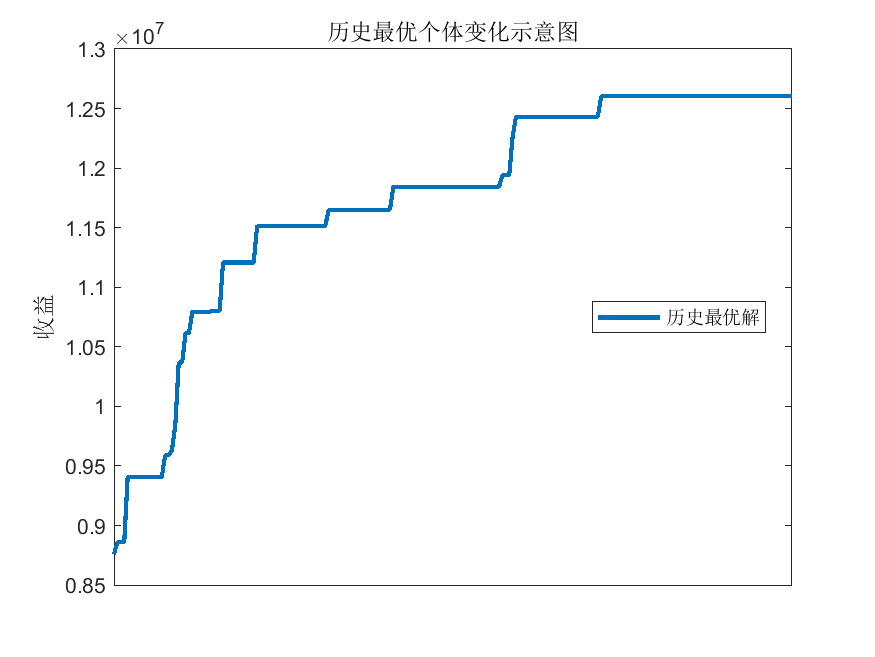
\includegraphics[width=11cm]{figures/历史最优个体变化示意图.png}
	\caption{ }\label{img003}
\end{figure}

很显然，在最优个体的不断变化中收益逐渐达到了最大值并趋于稳定。模型最终求解效果很可观。
\subsection{问题二的模型建立与求解}
\subsubsection{数据处理与分析}
\begin{table}[!htbp]
	\caption{参数取值表}\label{tab002} \centering
	\begin{tabular}{|c|c|} 
		\hline
		参数名称                    & 取值     \\ 
		\hline
		小麦和玉米预期销售量的年平均增长率       & 5\%    \\ 
		\hline
		其他作物相对于2023年的预期销售量增长变化率 & -5\%   \\ 
		\hline
		农作物亩产量的年增长变化率           & -10\%  \\ 
		\hline
		农作物种植的成本年增长率            & 5\%    \\ 
		\hline
		蔬菜类作物销售价格的年增长率          & 5\%    \\ 
		\hline
		食用菌类销售价格的年增长率           & -5\%   \\
		\hline
	\end{tabular}
\end{table}
对于不确定因素下的优化问题，本文采用鲁棒优化的方法，在最坏情况下目标函数的函数值达到最优，使得该解在可能出现的所有情况下，约束条件均能被满足，同时也增加了方案的可行性，减少了参数扰动对于种植策略的影响。

在题设条件下，选择最不利于目标函数取得较大值的参数大小，如表~\ref{tab002}~所示。

此外， 除了预期销售量、农作物亩产量、种植成本以及销售价格的不确定性，还有许多的潜在种植风险值得去考虑。近年来，受不断恶劣的极端气候影响，我国农作物受灾、成灾、绝收面积不断变化。

农作物受灾面积指：农作物比正常年份减产10％以上的播种面积。 （此处记作10\%）

农作物成灾面积指：农作物比正常年份减产30％及以上的播种面积。 （此处记作30\%）

农作物绝收面积指：农作物比正常年份减产70％及以上的播种面积。 （此处记作70\%）

据国家统计局编写的《中国统计年鉴2023》\cite{bib:one}数据表示，近十年来的自然灾害所导致的
受灾、成灾、绝收面积高居不下，具体如表~\ref{tab004}~所示：


\begin{table}[!htbp]
	\caption{近十年自然灾害导致受灾、成灾、绝收面积(单位：千公顷)}\label{tab004} \centering
	\begin{tabular}{|c|c|c|c|c|c|} 
		\hline
		年份   & 受灾面积    & 成灾面积   & 绝收面积    & 耕作面积      & 灾害损失率     \\ 
		\hline
		2023 & 10539   & 4797   & 980     & 171624.47 & 0.981     \\ 
		\hline
		2022 & 12072   & 4373   & 1351.8  & 169990.92 & 0.98      \\ 
		\hline
		2021 & 11739   & 4682   & 1632.8  & 168695.13 & 0.978     \\ 
		\hline
		2020 & 19958   & 7993   & 2706    & 167487.14 & 0.962     \\ 
		\hline
		2019 & 19257   & 7913   & 2802    & 165930.66 & 0.962     \\ 
		\hline
		2018 & 20814   & 10569  & 2585    & 165902.38 & 0.957     \\ 
		\hline
		2017 & 18480   & 9200   & 1826.7  & 166331.91 & 0.965     \\ 
		\hline
		2016 & 26220   & 13670  & 2902.2  & 166939.04 & 0.948     \\ 
		\hline
		2015 & 21770   & 12380  & 2232.7  & 166829.28 & 0.955     \\ 
		\hline
		2014 & 24890   & 12680  & 3090.3  & 165183.32 & 0.949     \\ 
		\hline
		平均值  & 18573.9 & 8825.7 & 2210.95 & 167491.4  & 0.963749  \\
		\hline
	\end{tabular}
\end{table}

灾害损失率的计算方法如下：
灾害损失率=(耕作面积-10\%$\times$受灾面积-30\%$\times$成灾面积-70\%$\times$绝收面积)/耕作面积$\times$100\%

在此基础上，为了反映自然情况下的灾害损失率大小，预想构造满足某正态分布的随机量，以得到不同年份下的灾害损失率。
然后针对灾害损失率随机量进行夏皮洛-威尔克检验，判断在95\%的置信水平下，是否能拒绝原假设$H_0$：该随机量服从正态分布。正态性检验结果位于\underline{附件}中，得到无法拒绝原假设的结果，所以灾害损失率随机量服从期望为0.9637，方差为0.00151的正态分布，即$X\sim N(0.9637,0.000151)$。最后以此为依据生成不同年份下的灾害损失率，与产量相乘参与计算。

\subsubsection{模型建立}
在算法设计上，基本沿袭第一问的算法。对于超出预期销售量的部分同第一问的第一种情况进处理，即超过部分滞销，造成浪费。同时对将目标函数修改为如下：

\begin{equation*}
	\begin{split}
	W_1&=\sum_{i}^{54} \sum_{j}^{4}min(\frac{ \text{Yield}_{m,n} \times \text{Field}_{i,5}}{2}\times 0.9^{t-2023} ,\text{Sale}_{m,n}\times 0.95
	)\times \text{Price}_{m,n}\times 1.05^{2023-t}\\
	&-\frac{ \text{Cost}_{m,n}\times \text{Field}_{i,5}\times 1.05^{t-2023}}{2}   
	\end{split}
\end{equation*}	

其中，$m=\text{Field}_{i,j},n=\text{Field}_{i,6}$。$t$表示年份。
此处参数设置仅对大部分作物与地块有效，部分特殊对象在算法中单独进行处理

\subsubsection{模型求解}
运用问题一编写的python模型，修正目标函数，将数据带入模型进行求解，得到此刻情况下2024-2030年的最优农作物种植方案。最终方案已经存入result2.xlsx，置于支撑材料中。

\subsection{问题三的模型建立与求解}
\subsubsection{数据相关性分析}
\begin{table}[!htbp]
	\caption{描述统计}\label{tab003} \centering
	\begin{tabular}{|c|c|c|c|c|c|c|} 
		\hline
		& 最小值  & 最大值    & 均值           & 方差            & 偏度     & 峰度\\ 
		\hline
		种植成本/(元/亩) & 350  & 10000  & 1890.65   & 3636363.511   & 2.605  &9.143\\ 
		\hline
		销售单价/(元/斤) & 1.50 & 100.00 & 9.0742    & 205.306       & 5.137  &28.946\\ 
		\hline
		预期销售量/斤    & 810  & 150000 & 20165.89  & 780961176.659 & 2.553  &7.966\\
		\hline
	\end{tabular}
\end{table}

为了得到预期销售量、销售价格和种植成本之间的相关性，我们选取附件提供的2023年各类农作物的相关数据进行数据分析，有表~\ref{tab003}~所示结果。

很明显农作物的三类统计量都出现方差、偏度、峰度较大的现象。尤其是销售单价一栏，反映出农作物单价分布不对称，高价农作物占多，拉动整体价格水平；并且整体分布不均匀，稳定性很差。这跟当地作物多样性，作物属性关系联系很大。

然后检验三类数据是否属于正态分布数据，由于样本数较大，所以我们采取JB检验去判断数据是否属于正态分布。即我们假设他们各自都属于正态分布，分别计算它们对应的p值。通过matlab计算得到它们的p值都是$10^{-3}$量级的，远小于0.05。故拒绝原假设，这三类统计量都不遵循正态分布。同时，我们做出了QQ图加以佐证，它们并不遵循正态分布。图~\ref{img005}~仅列出销售单价的qq图及其去趋势图。

\begin{figure}[htb]
	
	\begin{minipage}{0.5\linewidth}%可修改0.49为其他比例，调整大小
		%\vspace{3pt}
		\centerline{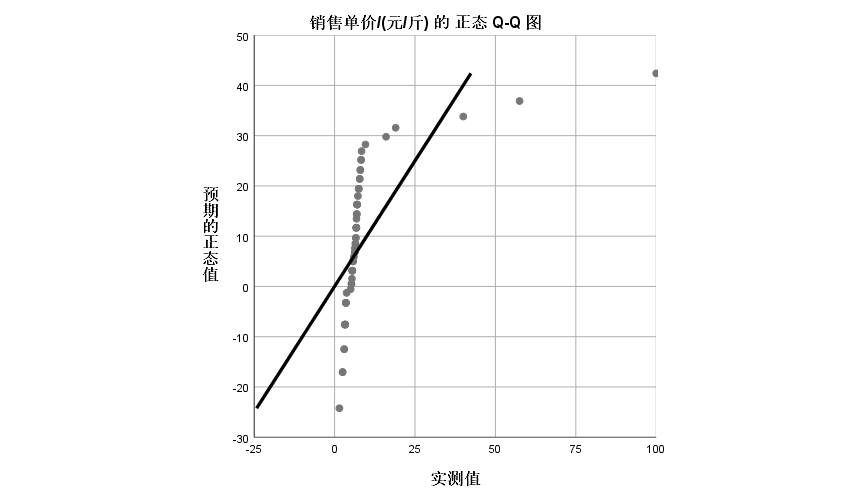
\includegraphics[width=10cm]{figures/qq图及其去趋势图2.png}}
	\end{minipage}
	\begin{minipage}{0.5\linewidth}
		%\vspace{3pt}
		\centerline{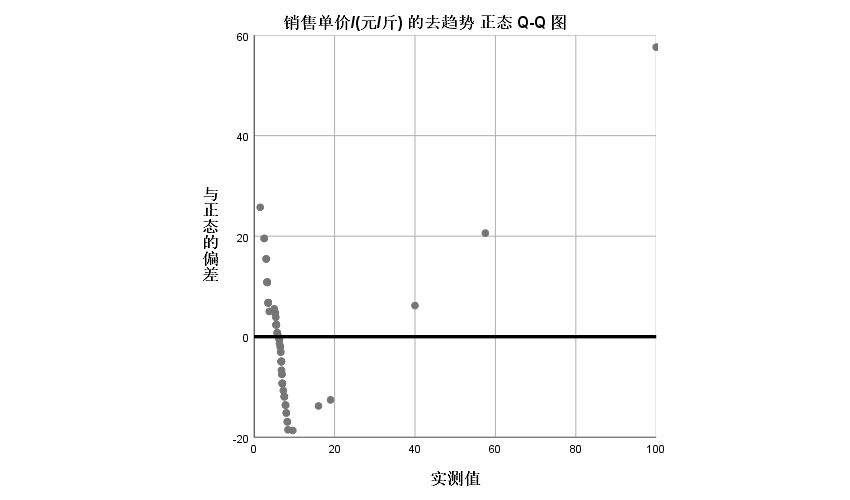
\includegraphics[width=10cm]{figures/qq图及其去趋势图3.png}}
	\end{minipage}
	
	\caption{销售单价qq图及其去趋势图}\label{img005}
\end{figure}

\begin{figure}[!htb]
	\centering
	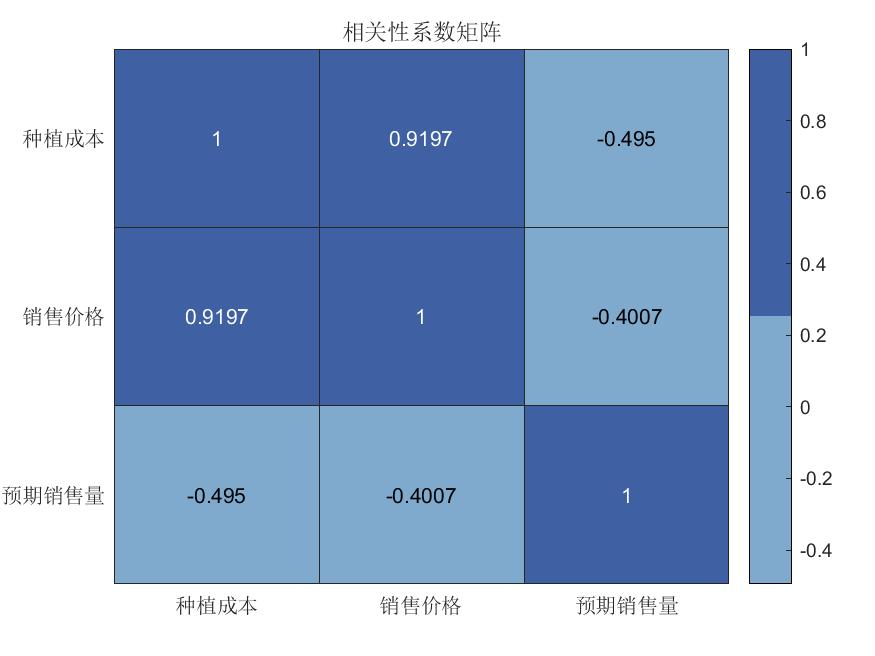
\includegraphics[width=11cm]{figures/斯皮尔曼相关系数.jpg}
	\caption{斯皮尔曼相关系数图}\label{img006}
\end{figure}

所以我们最终选择了斯皮尔曼相关系数来判断这三类统计量两两之间的相关性。如图~\ref{img006}~所示。

由图可知，种植成本和销售价格有很强的正相关性，种植成本与预期销售量呈负相关现象。

\subsubsection{直接曲线拟合}

由图~\ref{img006}~得到，种植成本和销售价格与预期销售量具有相关性。所以我们首先打算直接把种植成本与另外两个统计量进行函数拟合，去观察拟合优度如何。

由于三个统计量都属于经济数据，一般都具有异方差性，所以选择对数变化进行函数拟合，使得数据的方差更为稳定，提高拟合的准确性。同时，经过实际拟合证明对数变化后拟合优度确实高于线性回归。直接进行对数拟合的示意图如~\ref{img007}~所示。

\begin{figure}[h]
	\centering
	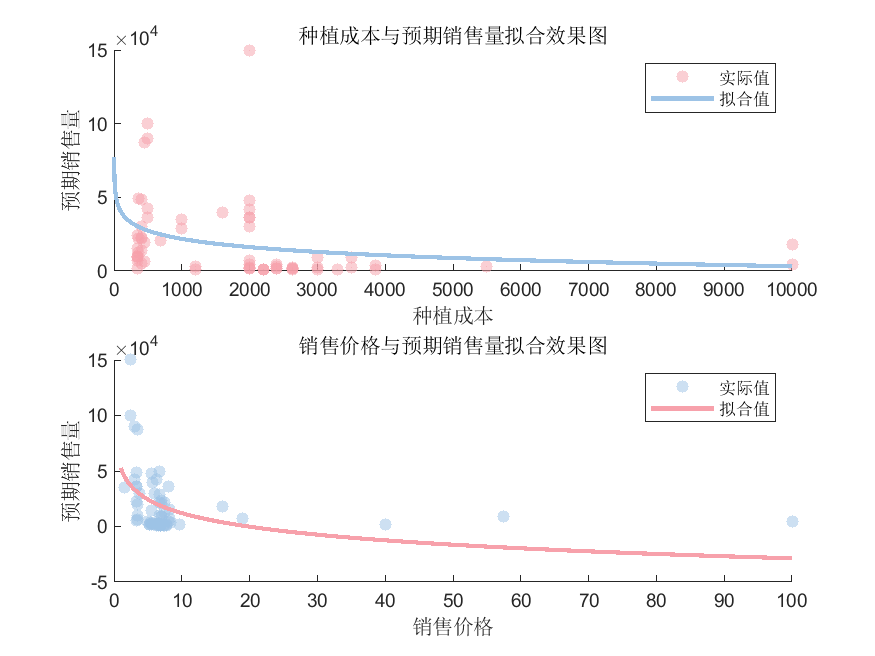
\includegraphics[width=11cm]{figures/直接拟合效果图.png}
	\caption{直接拟合效果图}\label{img007}
\end{figure}

虽然拟合效果相较于线性回归拟合好很多，但是相对于真实数据来说，直接进行对数拟合优度还是很低。种植成本与销售量拟合的曲线优度R方只有0.0777，销售单价与预期销售量拟合曲线的R方也只有0.1829。R方的值都过小，说明拟合效果还是很差。

\subsubsection{聚类分析后进行曲线拟合}
经过思考以及数据检验，发现极有可能是某些农作物性质区别过大引起的。因为一些农作物是生活必需品，哪怕成本不变，单价提高，预期销量浮动不会很大。而某些农作物属于高端奢侈品，销量受单价影响极为严重。因为这种极为对立的性质，所以我们放弃了直接进行曲线拟合，而是采取先对农作物进行聚类分析，将他们按照各自属性分类再进行各自类别相关统计量的曲线拟合。

为了对农作物进行分类，我们采用了系统聚类方法\textbf{中K-means++算法}通过种植成本和销售单价对农产品进行聚类。

\begin{figure}[h]
	\small
	\centering
	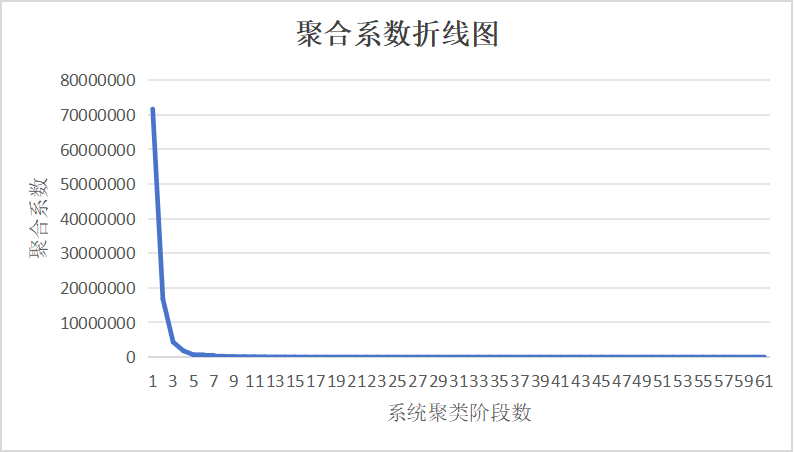
\includegraphics[width=11cm]{figures/聚合系数折线图.png}
	\caption{ }\label{img008}
\end{figure}

如图~\ref{img008}~所示，系统聚合系数不断迭代优化，到第5次的时候聚合系数趋于稳定，可以停止迭代。此时，通过\underline{附录}中聚合谱系图中可以看出，第五次迭代得到了三个聚类中心，即把农作物分成了三类。

matlab求解得到作物分类结果置于\underline{附录D}中，分类后发现其中第三类农作物只有两种，作物编号分别是200和41。这两种作物的显著特征是种植成本特别高，达到了10000元/亩。第一类农作物的种植成本较高，第二类农作物的种植成本偏低。因为第三类作物较少，种植成本接近第一类，所以我们将第三类农作物并进第一类以简化模型。
\begin{figure}[h]
	\centering
	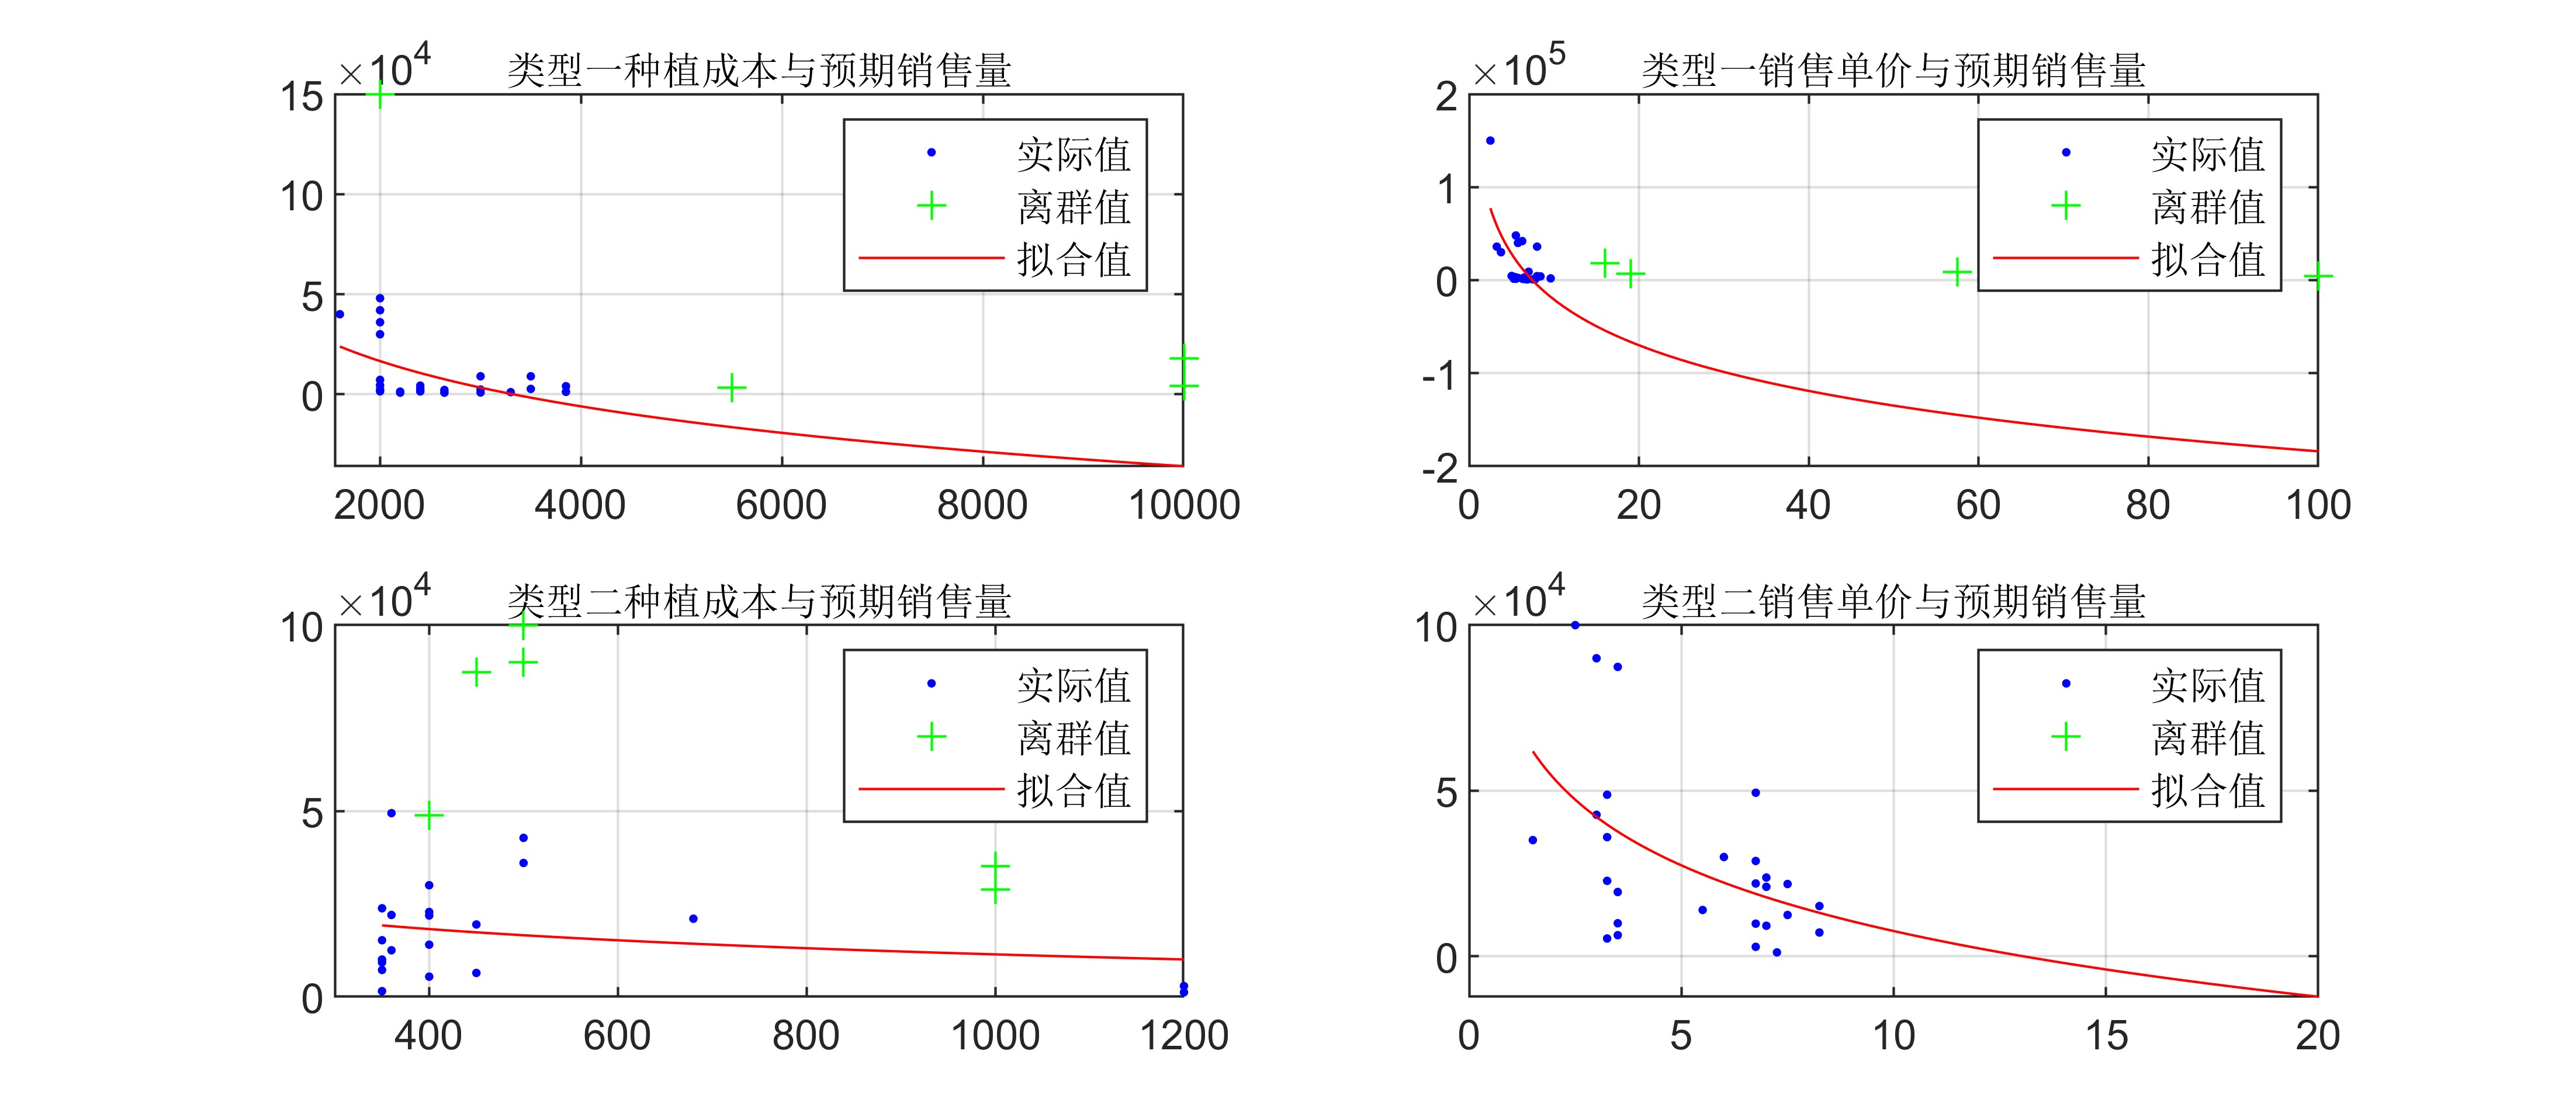
\includegraphics[width=15cm]{figures/曲线拟合图.jpg}
	\caption{聚类后农作物相关统计量曲线拟合图}\label{img010}
\end{figure}

所以，最终将农作物分成了两类种植成本较高的记为I类，较低的记为II类。对这两类植物分别进行
成本与销售量等相关曲线的拟合。拟合效果很好，单对于销售单价与销售量而言，两类作物的拟合优度R方相比于直接拟合分别提高了144.1\%,32.9\%。图~\ref{img010}~是分类之后的相关曲线拟合图。

\subsubsection{模型建立求解}

得到作物成本，单价和销量的之间的关系后。为了在问题二的基础上综合考虑相关因素，我们保持农作物成本与问题二使用的成本保持一致。因为成本属于比较稳定的因素，变动较小。此时我们通过拟合好的函数可以计算出农作物该成本下对应的单价和销量。此时，所建立的模型相较于第二问，单价和销量受函数关系影响发生了改变。同时，为了避免销量过剩，约束条件中使得销量总满足小于等于预期销量。此时，输入数据，用Python进行模型求解即可得到2024-2030年农作物的最优种植方案。

\subsubsection{比较分析}

为简化计算与数据复杂度，此处我们仅列出第二问和第三问分别所得到的2024年在34个地块所做的农作物最优种植策略进行比较。具体数值如图~\ref{img002}~所示。
\begin{figure}[h]
	\small
	\centering
	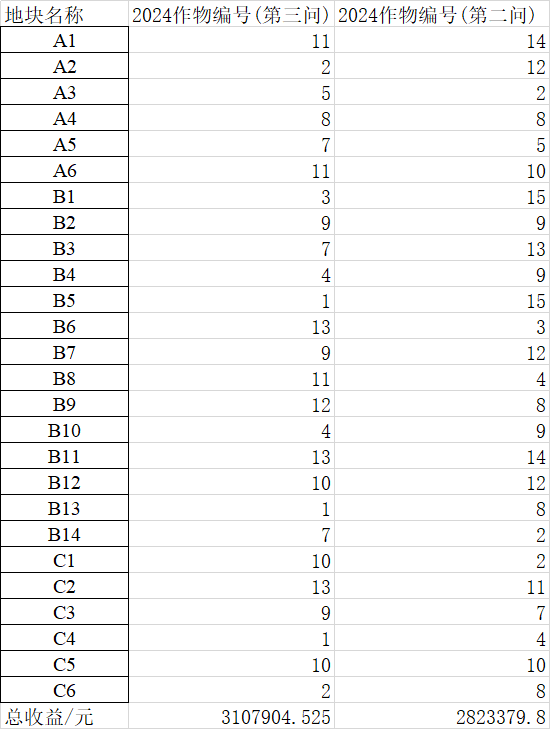
\includegraphics[width=9cm]{figures/compare.png}
	\caption{ }\label{img002}
\end{figure}

第三问通过挖掘各个指标之间的相关性得到拟合函数，以种地成本对预期销售量进行估计，便于对产量的把控，避免出现供给远超需求的情况，避免了产品浪费，也使得销售利润提升。

比较由第二问第三问的相关利润数据可以清楚地观察到，在将指标相关性纳入考虑后，产品总收益的提升，且各作物产量与预期销售量的差异减小，相当程度上降低了产品滞销问题发生的可能。
\section{结果分析与模型评价}
\subsection{模型检验及可靠性分析}
\subsubsection{模型检验}

\textbf{数据验证}：首先，我们对输入模型的历史销售数据进行了严格的验证，确保数据的准确性、完整性和一致性。通过对比不同来源的数据（如收银系统、库存管理系统等），我们排除了潜在的数据错误和异常值，确保模型输入数据的质量。

\textbf{模型拟合度检验}：对于使用曲拟合技术建立的销售量与平均价格之间的关系函数，我们进行了拟合度检验。通过计算残差平方和、决定系数（R²）等指标，我们评估了模型的拟合效果。结果显示，模型具有较高的拟合度，能够较好地反映销售量与价格之间的实际关系。

\textbf{预测准确性验证}：为了验证预测模型的准确性，我们将预测结果与后续实际销售数据进行了对比。通过计算预测误差率、均方误差（MSE）等指标，我们评估了预测模型的精度。结果显示，预测模型在多数情况下能够准确预测销售量，为补货与定价策略的制定提供了可靠依据。

\textbf{敏感性分析}：为了评估模型对参数变化的敏感性，我们进行了敏感性分析。通过调整关键参数（如成本、损耗率、价格上下限等），我们观察了模型输出结果的变化情况。结果显示，模型对参数变化具有一定的鲁棒性，能够在一定范围内保持稳定的输出结果。

\subsubsection{可靠性分析}

\textbf{算法稳定性}：我们选择的遗传算法等启发式搜索算法具有全局搜索能力强、鲁棒性好的优点。通过多次运行算法并观察结果的一致性，我们验证了算法的稳定性。结果显示，算法在多次运行中均能找到较为接近的最优解，证明了其可靠性。

\textbf{数据依赖性分析}：我们分析了模型对数据的依赖程度，并评估了数据质量对模型输出结果的影响。结果显示，模型对数据质量有一定的容忍度，但在数据质量较差的情况下，模型输出结果可能会出现较大偏差。因此，我们强调了数据治理的重要性，以确保模型输入数据的质量。

\textbf{约束条件合理性}：我们对模型中的约束条件进行了合理性分析。通过对比实际运营情况与约束条件设置，我们验证了约束条件的合理性和有效性。结果显示，约束条件能够较好地反映实际运营中的限制条件，为模型求解提供了有力的支持。

\subsection{模型评价与推广}
\subsubsection{模型优点}
\textbf{实用性}：本模型针对生鲜商超的运营需求，提供了科学的补货量与定价策略，显著提升了运营效率与盈利能力。然而，在实际应用中，商超仍需根据自身具体情况对模型进行适当调整，以确保其完全贴合实际运营需求。

\textbf{准确性}：模型在数据验证、拟合度检验及预测准确性方面表现良好，但也存在一定的局限性。例如，当销售数据受到异常事件（如天气突变、疫情等）影响时，模型的预测准确性可能会受到一定影响。因此，在实际应用中，商超需要密切关注市场动态，及时调整模型参数，以提高预测准确性。

\textbf{灵活性}：模型具有较高的灵活性，可根据商超的实际需求进行调整。但同时，这也对商超的数据分析和运营能力提出了较高要求。商超需要拥有专业的数据分析团队和先进的数据分析工具，以支持模型的持续优化和迭代。

\subsubsection{缺陷与改进}

\textbf{数据依赖性}：模型对数据质量要求较高，若数据存在缺失、错误或异常值，将直接影响模型的准确性和可靠性。因此，建议商超加强数据治理工作，建立完善的数据质量控制体系，确保数据的准确性和完整性。

\textbf{预测精度限制}：由于市场环境的复杂性和不确定性，模型在预测精度上仍存在一定的局限性。为提高预测精度，可以考虑引入更多的数据源（如社交媒体数据、天气预报等）和更先进的预测算法（如深度学习等），以丰富模型的信息输入和算法能力。

\textbf{约束条件灵活性}：模型中的约束条件是基于当前运营情况设定的，但未来随着商超的发展和市场环境的变化，这些约束条件可能需要进行调整。因此，建议商超定期评估模型约束条件的合理性，并根据实际情况进行必要的调整和优化。

\subsubsection{模型推广}
在克服了上述缺陷并进行了相应的改进后，本模型具有较高的推广价值。一方面，它可以应用于其他零售行业和供应链管理领域，通过调整模型参数和约束条件来适应不同行业的运营特点和需求；另一方面，通过技术升级和合作共享等方式，可以进一步提升模型的智能化水平和预测准确性，为相关企业提供更加精准的决策支持。同时，我们也鼓励商超之间加强合作与交流，共同推动零售行业的数字化转型和智能化升级。

%参考文献
\begin{thebibliography}{9}%宽度9
	\bibitem{bib:one}《中国统计年鉴2023》编委会和编辑出版人员　《中国统计年鉴2023》编委会和编辑出版人员. 付凌晖,叶礼奇 总编,中国统计年鉴,中国统计出版社,2023,4-5,年鉴.
\end{thebibliography}
\newpage
%附录

\begin{appendices}
\section{支撑材料文件列表}
\begin{table}[!htbp]
	\centering
	\begin{tabular}{ccc}
		\toprule[1.5pt]
		文件 & 类型 & 简介  \\
		\midrule[1pt]
		
		.py & python代码文件 & 代码 \\
		.py & python代码文件 & 代码 \\
		.py & python代码文件 & 代码 \\
		.py & python代码文件 & 代码 \\
		.py & python代码文件 & 代码 \\
		\bottomrule[1.5pt]
	\end{tabular}
\end{table}

\section{问题一相关代码和处理结果}

\end{appendices}

\end{document} 